\subsection{Caspar}%
\label{sub:caspar}

\begin{wrapfigure}[13]{R}{0.35\textwidth}
    \centering
    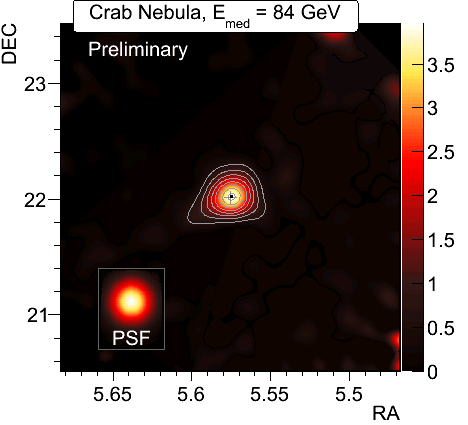
\includegraphics[width=\linewidth]{pictures/skymap.png}
    \caption{Diese Skymap will durch ein passendes Bild ersetzt werden.}%
    \label{fig:skymap}
\end{wrapfigure}

Skymaps sind Grundlage einer jeden Datenanalyse
und sind von besonderem Interesse bei ausgedehnten Quellen.
Durch das Vermessen von ausgedehnten Quellen
lässt sich beispielsweise der Zeitpunkt einer Supernova-Explosion schätzen.

\paragraph{Theorie}%
\label{par:theorie}

Eine Skymap ist eine zweidimensionale Repräsentation der aufgenommen Photonen.
Ziel ist es, den gemessenen Events eine Position zuzuordnen.
Dazu werden ge\-wöhn\-lich drei verschieden Koordinatensysteme genutzt:

\begin{description}
	\item[\quad Kamera Koordinaten] werden genutzt, um die Sensitivität des
    Teleskops
		als eine Funktion in der Kamera zu beschreiben.
    Eine Repräsentation ist in Abbildung~\ref{fig:cleaning} zu sehen.
		Anhand dieser lassen sich beispielsweise Inhomogenitäten,
		wie sie ein helle Quelle verursacht, bereinigen.

	\item[\quad Azimuthal Koordinaten] sind abhängig von der Position des
		Beobachters auf der Erde.
		Sie sind nicht für die Observation von Astronomischen Objekten von Nutzen,
		aber um die Performance zu testen.
		Dazu werden Daten bei verschiedenen Zenitwinkel verglichen,
    was eine Variation der Atmosphärendicke entspricht.

	\item[\quad Equatorial Koordinaten] werden genutzt um eine Skymap einer
		astrophysikalischen Quelle anzufertigen.
    % {\color{red} Noch beschreiben wie es aussieht.}
\end{description}

Die Anfertigung einer Skymap ist nicht so simpel wie bei einem gewöhnlichen
Bild.
Für eine Skymap reicht nicht allein die Konstruktion eines 2D-Arrays,
bei dem die Information allein im Signalverlauf der Pixel enthalten ist,
wie es bei gewöhnlichen Bildern der Fall ist.

Vielmehr wird für jedes Gammaevent ein einzelnes Bild aufgenommen,
auf dem die Richtung rekonstruiert wird.
Eine Skymap bildet eine Menge an rekonstruierten Richtungen im Himmel ab.
Da die Richtungskonstruktion der Events einen gewissen Fehler aufweist,
schmieren die rekonstruierten um die wahren Quellposition aus.
Das Ausschmieren der Quelle wird durch die \textit{Point Spread Function (PSF)}
beschrieben
und kann auf einer Skymap bestimmt werden.
Durch die PSF kann das Auflösungsvermögen eines Teleskops
beschrieben werden und bildet daher eine wichtige Größe.

\paragraph{Durchführung}%

Die Konfigurationsdatei \texttt{caspar.rc} wird verwendet.
Es muss das Feld \texttt{Caspar.dataName} angepasst werden.
Wie bei Odie werden die von Melibea prozessierten Daten genutzt.


\begin{lstlisting}
  caspar -q -b --config=caspar.rc
\end{lstlisting}
